\chapter{Evaluation} 
\label{sec.evaluation}
In this section, we demonstrate SOAR's utility by implementing two example use cases that together play different types of its API: comparing the performance of 2.4 GHz and 5 GHz bands and studying channel survey statistics. Our goal is to illustrate how \sysname can support a variety of measurement needs.
\section{Usecase: Comparing the wireless performance of 2.4 and 5GHz bands}
\label{sec.usecase1}
Better use of 5 GHz to improve wireless performance on a dense WiFi network is a common strategy because there are generally fewer devices in the 5 GHz band (This means that the noise floor is much lower) and 5 GHz band has less non-WiFi interference. Thus our hypothesis was that devices on the 5 GHz band would perform better.
\newline
We use \sysname to evaluate the wireless performance of network traffic on 2.4 GHz and 5 GHz band. Our focus is not on improving performance, but rather to underscore how we can use \sysname to gain useful insights into a real network.
For our experiment, the router that we use has both 2.4 GHz and 5 GHz radios, which allows us to compare the performance of these two bands. To ensure there are similiar network traffic on 2.4 GHz and 5 GHz band, we performed a multi-threaded TCP experiment on \sysname to send intermittent TCP packets to clients which connected 2.4 GHz and 5 GHz band respective. Then we collect network traffic statistics to compare wireless performance of network.

\begin{figure}
\begin{subfigure}{0.5\textwidth}
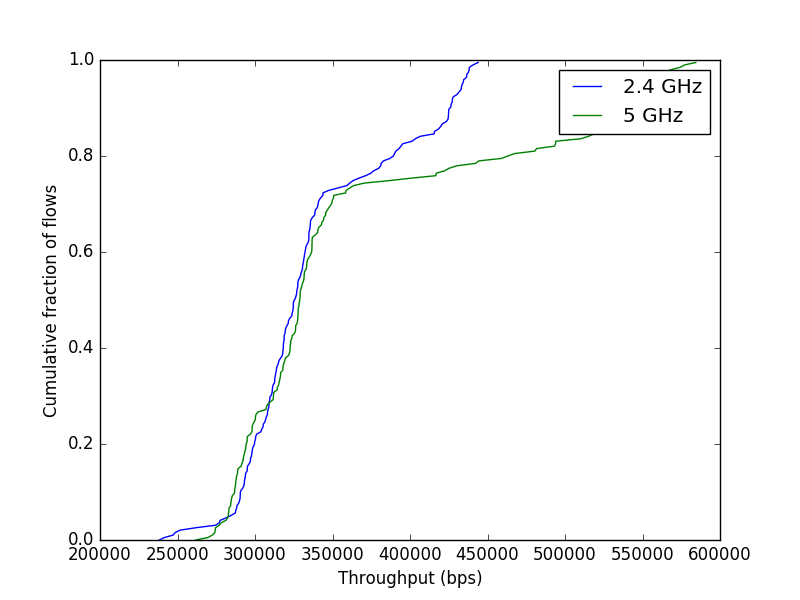
\includegraphics[width=\linewidth]{figure/throughput(5g_vs_2g).png}
\caption{Network traffic in the 5 GHz band achieve higher throughput} 
\label{fig:throughput}
\end{subfigure}
\hspace*{\fill} % separation between the subfigures
\begin{subfigure}{0.5\textwidth}
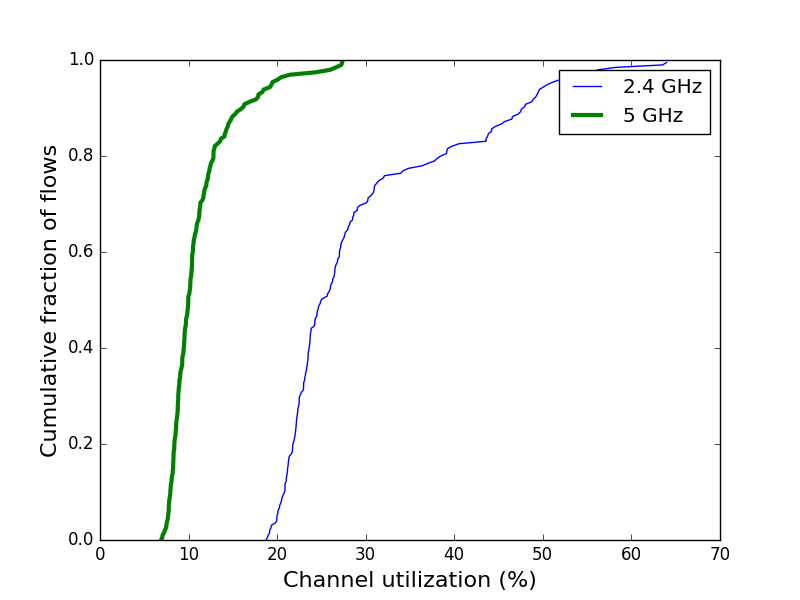
\includegraphics[width=\linewidth]{figure/channel_utilization(2g_vs_5g).png}
\caption{Network traffic in the 2.4 GHz band experience higher channel utilization.} 
\label{fig:utilization}
\end{subfigure}
\hspace*{\fill} % separation between the subfigures
\begin{subfigure}{0.45\textwidth}
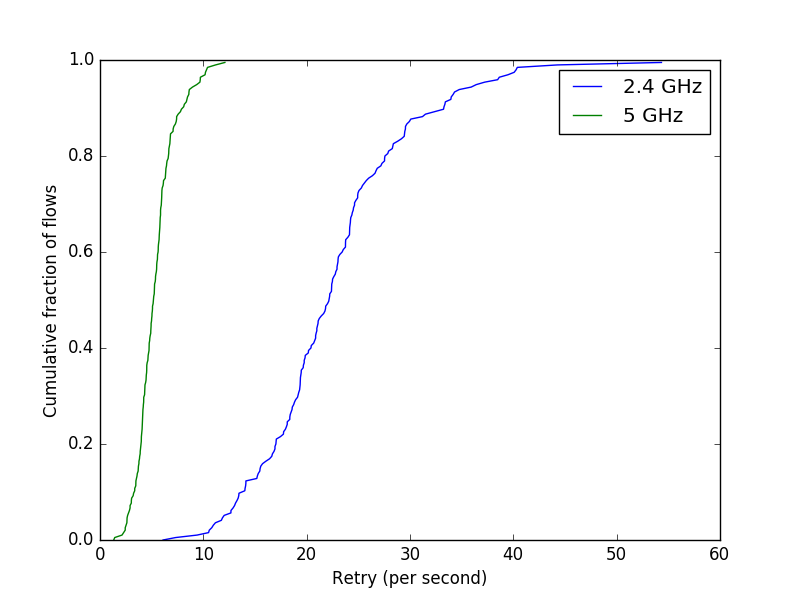
\includegraphics[width=\linewidth]{figure/retries(2g_vs_5g).png}
\caption{Network traffic in the 2.4 GHz band experience higher tx retries.} 
\label{fig:retries}
\end{subfigure}
\hspace*{\fill} % separation between the subfigures
\begin{subfigure}{0.5\textwidth}
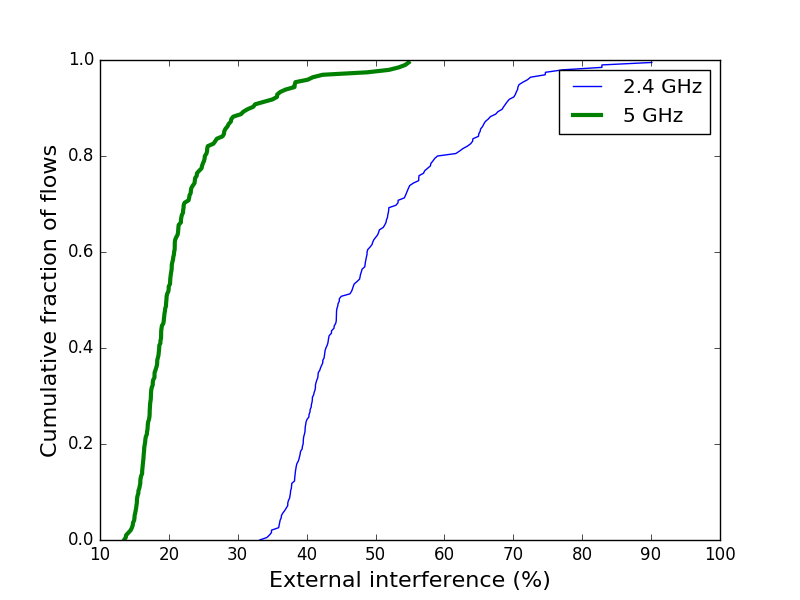
\includegraphics[width=\linewidth]{figure/external_interference(2g_vs_5g).png}
\caption{Network traffic in the 5 GHz band has less external interference.} 
\label{fig:interference}
\end{subfigure}
\caption{Characteristics of flows in the 5 GHz vs. the 2.4 GHz spectrum.} 
\label{fig:5gvs2g}
\end{figure}

\textbf{The 5 GHz band performs better than the 2.4 GHz band.} We use throughput, channel utilization, retransmission times and external interference as our indicator of wireless performance because we can obtain these metrics easily from our supported APIs. We calculate throughput as follows: using \textit{get\_network\_bytes} to provide TCP statistics. We study the aggregate TCP throughput achieved during the captured lifetime of the network traffic. We compute the average throughput at every one-second interval by the divisor of aggregate TCP throughput and the difference between the correspond timestamp. \textit{get\_station} can help us obtain the number of retry packets at each clients. We also compute channel utilization and external interference as the percentage of channel busy time and external interference time in any given one-second interval. 
\newline
We see that 5 GHz has a better performance. Figure \ref{fig:throughput} shows the network traffic in the 5 GHz band achieve higher throughput. Figure \ref{fig:utilization} shows the channel utilization in 2.4 GHz are much higher than 5 GHz. Figure \ref{fig:retries} shows the retransmission times per 40 seconds; the result shows that transmissions are more common in the 2.4GHz band. Figure \ref{fig:interference} plots the CDF of the external interference for all network traffic for both the 2.4 GHz band and the 5 GHz bands. The 5GHz band has less interference as signal does not propagate well through walls.

\begin{figure}
\centering
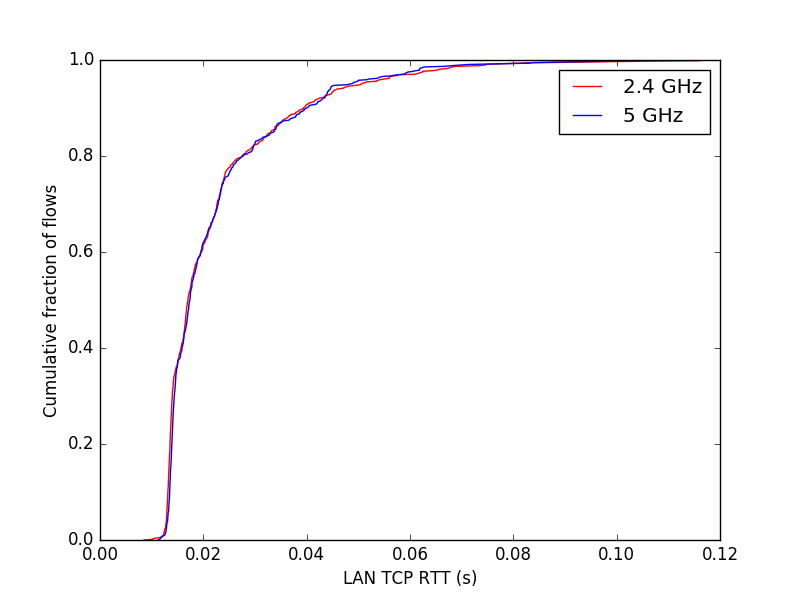
\includegraphics[width=0.5\textwidth]{figure/tcp_rtt.png}
\caption{LAN TCP round-trip time for different bands. } 
\label{fig:tcprtt}
\end{figure}

\textbf{TCP round-trip time is similar on 2.4 GHz and 5 GHz band.} We calculate TCP round-trip time as follows: using the home router as vantage point and calculate the time between a TCP packet coming and its respective TCP acknowledgement from a connected client. We collected the TCP round-trip between the wireless home router and a wireless client on 2.4 GHz and 5 GHz band. Figure \ref{fig:tcprtt} plots the CDF of the TCP round-trip times for all network traffic for both the 2.4 GHz band and the 5 GHz bands. The result shows that TCP round-trip time on 2.4 GHz and 5 GHz band are similar.

\textbf{Within a home network, individual devices can experience different wireless performance at different time.} Figure \ref{fig:compare} uses the WiFi data set to show throughput of wireless network during each hour of day, partitioned into weekday and weekend. We observe a diurnal throughput in home network in a office building at various times of day on a weekday and weekend. We see that throughput is higher at weekend than weekday, which may result from there are less external interference (e.g., surrounding access points, clients).

\begin{figure}
\centering
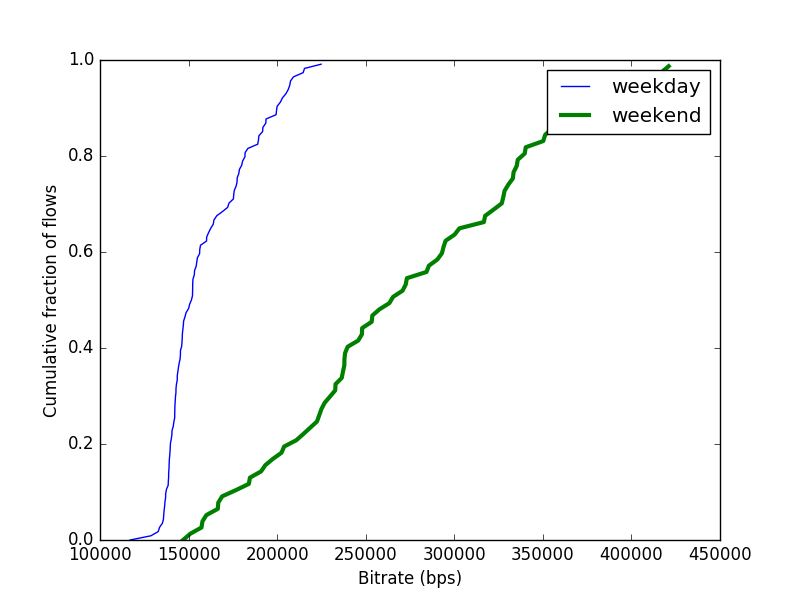
\includegraphics[width=0.5\textwidth]{figure/bitrate(weekday_vs_weekend).png}
\caption{Bitrate on weekday and weekend. Weekend bitrate is more than weekday bitrate.} 
\label{fig:compare}
\end{figure}  

\section{Usecase: Studying channel survey statistics}
\label{sec.usecase2}

\begin{figure}
\centering
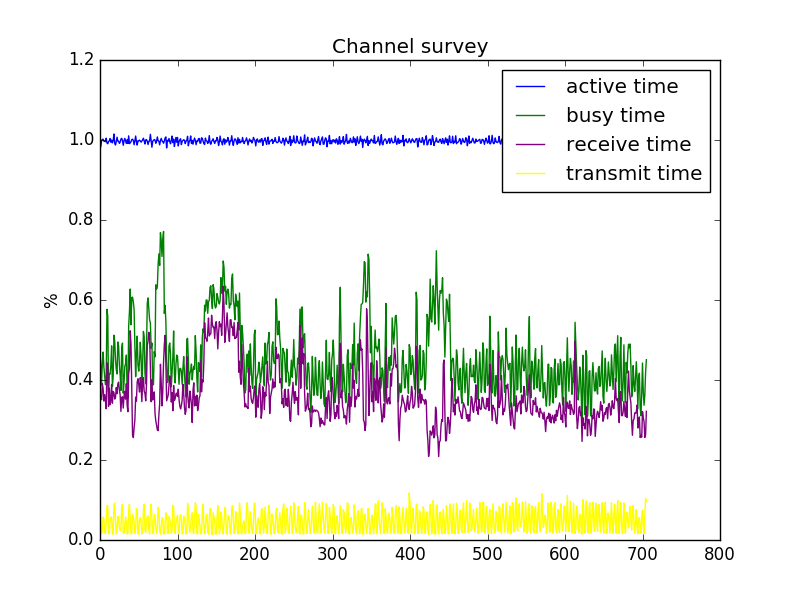
\includegraphics[width=0.5\textwidth]{figure/channel.png}
\caption{Channel survey.} 
\label{fig:channelsurvey}
\end{figure}
Measurement studies show that congestion in a wireless network leads to lower overall network throughput and capability. The lack of techniques to identify and characterize congestion in wireless networks has prevented relevant research. To better understand congestion in wireless networks, \sysname provides the capabilities to explore radio channel channel utilization data. 
\newline
As \cite{channelsurvey} did before, we replicated this experiment through our \sysname platform. We use \textit{wifi\_status} to collect channel busy time, active time, transmit time and receive time. Figure \ref{fig:channelsurvey} shows the channel survey statistics captured in 2.4 GHz band. We find that channel active time is the same as running time if you don't change channels. Channel busy time seems to be the same as the sum of transmit time and receive time, unless there is a lot of external interference (e.g, heavy external traffic on the same channel, non-WiFi devices).
